\documentclass{article}
\usepackage{graphicx} % Load the graphicx package
\usepackage{amsmath} % Required for math symbols like \frac


\begin{document}
\title{Exercício 10} 
\author{Arthur Felipe Reis Souza}
\date{\today}
\maketitle





\section{Introduction}

\vspace{10pt}

O exercício semanal consiste em utilizar diferentes arquiteturas das redes MLP, de forma a resolver um problema de regressão e um problema de classificação. O dataset de classificação é o dataset Statlog, que consiste em um conjunto de características de um indivíduo que serão utilizadas para classificar a presença ou não presença de uma doença cardíaca. O dataset de regressão é o BostonHouse, que terá suas características utilizadas para estimar o valor médio de um imóvel em Boston.

\vspace{10pt}

A critério de comparação, no problema de classificação será utilizado dois algoritmos de Machine Learning para comparar o desempenho da rede MLP. Um será o classificado de Bayes e o outro o KNN.

\vspace{10pt}

\section{Desenvolvimento}

\vspace{10pt}

A primeira base de dados a ser utilizado é o BostonHouse, que inicialmente foi tratada usando o StandardScaler da biblioteca scikitlearn, normalizando todas as características do dataset. Após a normalização, foi utilizado o Grid-Search para encontrar o número de neuronios intermediários que levam ao modelo a uma melhor performance.

\vspace{10pt}

\begin{figure}[h]

    \centering
    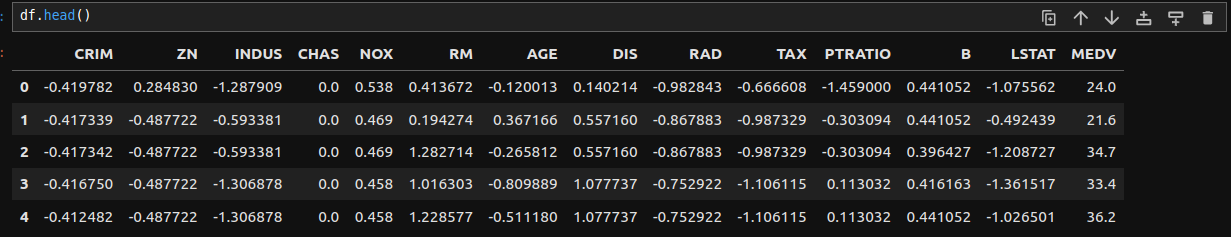
\includegraphics[height=1in]{dados_normalizados.png}
    \caption{Dados normalizados BostonHouse.}
    \label{fig:example}
    
\end{figure}

\vspace{10pt}

O mesmo foi realizado para o dataset Statlog.

\vspace{10pt}

\begin{figure}[h]

    \centering
    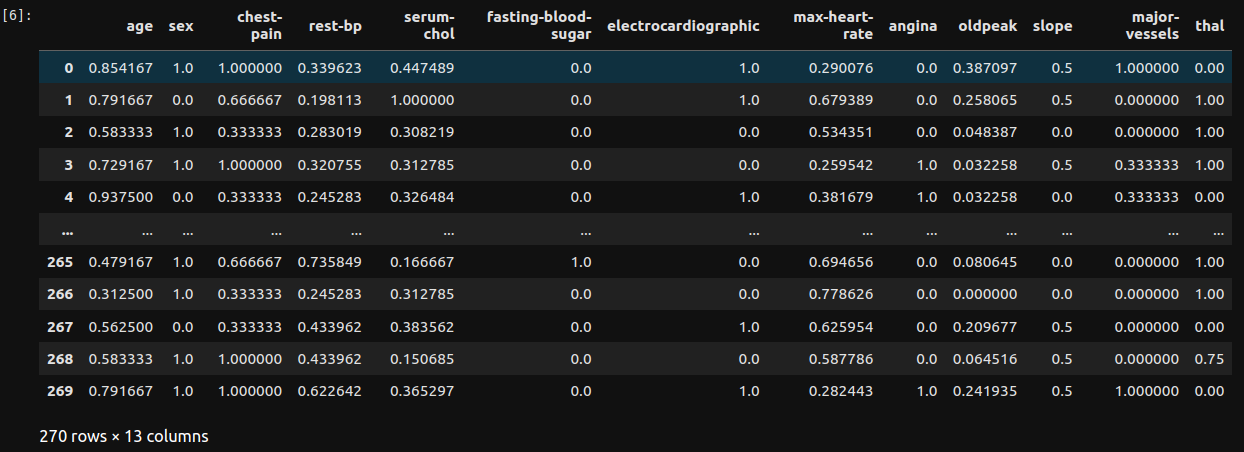
\includegraphics[height=1.5in]{normalized_data_statlog.png}
    \caption{Dados normalizados Statlog.}
    \label{fig:example}
    
\end{figure}

\vspace{10pt}



\vspace{10pt}

\section{Resultados}

\vspace{10pt}

\subsection{Boston House}

\vspace{10pt}

Os resultados para o dataset de regressão boston foram : 

\vspace{10pt}

\begin{figure}[h]

    \centering
    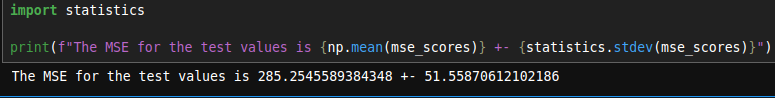
\includegraphics[height=0.5in]{reg_5n.png}
    \caption{Resultado usando 5 neuronios na camada intermediária com o otimizador ADAM.}
    \label{fig:example}
    
\end{figure}

\vspace{10pt}

\vspace{10pt}

\begin{figure}[h]

    \centering
    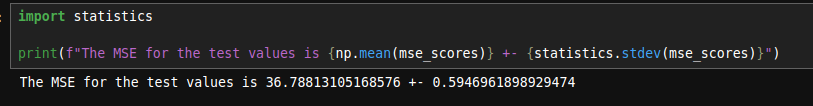
\includegraphics[height=0.5in]{best_reg.png}
    \caption{Resultado usando 40 neuronios na camada intermediária com o otimizador ADAM.}
    \label{fig:example}
    
\end{figure}

\vspace{10pt}


\vspace{10pt}

\begin{figure}[h]

    \centering
    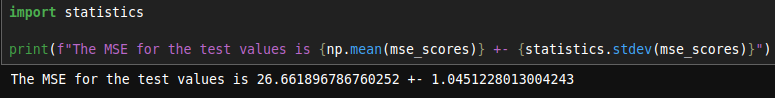
\includegraphics[height=0.5in]{10_neuron.png}
    \caption{Resultado usando 10 neuronios na camada intermediária com o otimizador Gradiente Estocástico e a técnica de early stopping.}
    \label{fig:example}
    
\end{figure}

\vspace{10pt}

\subsection{Statlog}

\vspace{10pt}

No dataset Statlog, por ser de classificação, também será avaliado pela métrica AUC (Area Under the Curve). Essa métrica tem por objetivo avaliar o desempenho de um classificador variando os valores de threshold. Quanto mais próximo de 1, melhor é o desempenho do mesmo. No exercício, como dito anteriormente, foram utilizados 3 diferentes classificador, o classificador de Bayes, o KNN e uma rede MLP. Os resultados do desempenho estão mostrados abaixo :     

\vspace{10pt}

\begin{figure}[h]

    \centering
    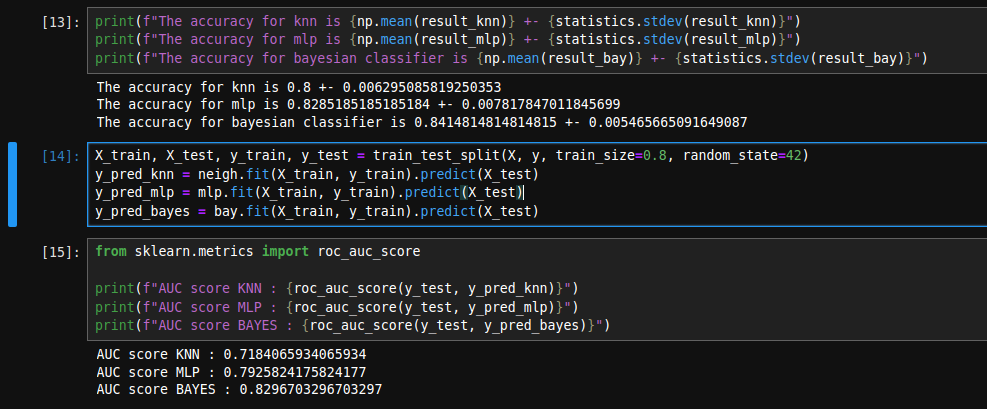
\includegraphics[height=1.5in]{result_1.png}
    \caption{Resultado usando 100 neuronios na camada intermediária com o otimizador ADAM, KNN com k=5, e o classificador de bayes.}
    \label{fig:example}
    
\end{figure}

\vspace{10pt}

\begin{figure}[h]

    \centering
    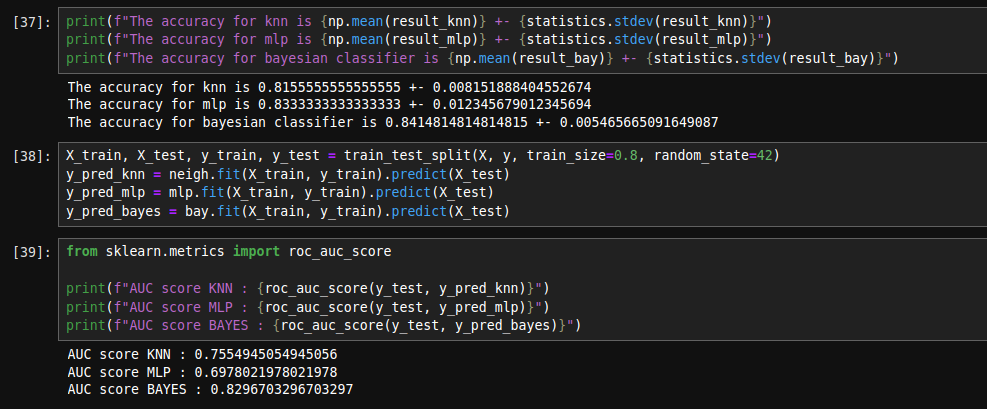
\includegraphics[height=1.5in]{result_2.png}
    \caption{Resultado usando 10 neuronios na camada intermediária com o otimizador ADAM, KNN com k=15, e o classificador de bayes.}
    \label{fig:example}
    
\end{figure}

\vspace{10pt}


\vspace{10pt}

\begin{figure}[h]

    \centering
    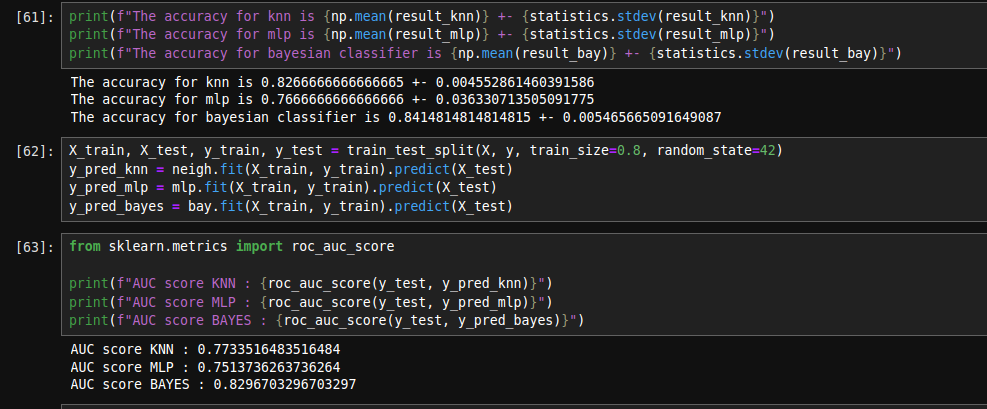
\includegraphics[height=1.5in]{result_3.png}
    \caption{Resultado usando 4 neuronios na camada intermediária com o otimizador ADAM, KNN com k=25, e o classificador de bayes.}
    \label{fig:example}
    
\end{figure}

\vspace{10pt}

\section{Conclusão}

\vspace{10pt}

Portanto, ao concluir com exito o exercício semanal no dataset de regressão e de classifcação, é possível afirmar que : No dataset Boston Housing, utilizando o mesmo otimizador, quanto maior o número de neurônios, menor o erro médio. Porém, ao alterar o otimizador para o gradiente estocástico e também utilizando a técnica de early stopping, o desempenho melhorou consideravelmente. No dataset Statlog, o classificador de bayes teve um desempenho relativamente melhor do que os outros dois algoritmos, mesmo realizando algumas variações nos hyperparâmetros do KNN e no MLP. O classificador de bayes é relativamente mais simples do que os outros dois algoritmos, e também teve uma melhor performance para essa base de dados.
\end{document}